\subsection{Tau Leptons}\label{sec:tau_reco}
\begin{table}
  \centering
  \begin{tabular}{llccc}
          \toprule
          & Decay mode & Resonance & \multicolumn{2}{c}{$\mathcal{B}$ (\%)} \\ 
          \midrule
          \multicolumn{2}{l}{Leptonic decays} & & 35.2 & \\
          & $\tau^- \to e^- \bar{\nu}_e \nu_\tau$ & & & 17.8 \\
          & $\tau^- \to \mu^- \bar{\nu}_\mu \nu_\tau$ & & & 17.4 \\
          \midrule
          \multicolumn{2}{l}{Hadronic decays} & & 64.8 & \\
          & $\tau^- \to h^- \nu_\tau$ & & & 11.5 \\
          & $\tau^- \to h^- \pi^0 \nu_\tau$ & $\rho(770)$ & & 25.9 \\
          & $\tau^- \to h^- \pi^0 \pi^0 \nu_\tau$ & $a_1(1260)$ & & 9.5 \\
          & $\tau^- \to h^-h^+h^ -\nu_\tau$ & $a_1(1260)$ & & 9.8 \\
          & $\tau^- \to h^-h^+h^- \pi^0 \nu_\tau$ & & & 4.8 \\
          & Other & & & 3.3 \\
          \bottomrule
  \end{tabular}
  \caption[Tau Lepton Decays and Branching Fractions]{Decays of $\tau$ leptons and their branching fractions ($\mathcal{B}$). Where appropriate, the known intermediate resonances for a decay are indicated. Charged hadrons are denoted by the symbol $h^\pm$ and although only $\tau^-$ decays are shown, the values are also valid for the charge-conjugated processes.}\label{tab:tau_decays}
\end{table}

Tau leptons decay into a variety of final states, which are summarized in \cref{tab:tau_decays}. About one third of the time, tau leptons decay \textit{leptonically} into an electron or muon, and two neutrinos. In such a decay, the electrons and muons are reconstructed as described in \cref{sec:eg_reco,sec:muon_reco}, and properties of the neutrinos are inferred from the missing transverse momentum. The other two thirds of the time, tau leptons decay \textit{hadronically} into hadrons and a neutrino. These types of tau leptons, denoted \tauh, are reconstructed with the hadrons-plus-strips (HPS) algorithm. 

\subsubsection{Hadrons-Plus-Strips Algorithm}

The HPS algorithm~\cite{CMS:2015pac,CMS:2018jrd} begins by searching the constituents of reconstructed jets for charged hadrons and neutral mesons. A $\pi^0$ meson promptly decays into two photons, which are then likely to convert into $e^+e^-$ pairs as they traverse the tracker material. The energy of the $\pi^0$ meson is therefore spread over a $\Delta\eta \times \Delta\phi$ region which is referred to as a \textit{strip}. The basic ingredients of the HPS algorithm are charged hadrons and strips, hence the name.

A strip is reconstructed by clustering electrons and photons inside a jet, and begins by seeding the strip with the highest \pt electron or photon in the jet. Then, a $\Delta\eta \times \Delta\phi$ area centred on the seed is defined and the next-highest \pt electron or photon inside the area is added to the strip. The strip position, which was originally defined by the seed, is then recomputed using a \pt-weighted average of all electrons and photons in the strip and the process is repeated until no more electrons or photons can be added.

The size of the $\Delta\eta \times \Delta\phi$ area is dynamic and is dependent on the \pt of the strip and of the candidate electron or photon to account for several effects~\cite{CMS:2018jrd}. Firstly, the likelihood of a photon converting into an $e^+e^-$ pair is higher at lower \pt, so the strip size is expected to be larger for lower \pt strips. Furthermore, the decay products for a \tauh with higher \pt tend to be boosted in the direction of the \tauh, leading to a smaller strip. The functions used to define the strip size are derived from simulation of \tauh decays and are designed such that 95\% of all electrons and photons arising from a \tauh decay are included in the strip.

Based on the set of charged hadrons and strips in a jet, the HPS algorithm identifies the decay mode from \cref{tab:tau_decays}. To reduce misidentification with jets, the mass of the sum of the hadron candidates is required to be compatible with a $\rho(770)$ or $a_1(1260)$ resonance, depending on the decay mode. Additionally, $\tau_h$ candidates are required to have a charge of $\pm1$, and to have no charged particles or strips outside a signal cone, defined by $R_{\text{sig}} = (3.0\GeV)/\pt$, where the \pt is that of the hadronic system, and the cone size is limited to 0.05--0.10. Finally, a single $\tau_h$ candidate is allowed per jet by selecting the candidate with the highest \pt. The \tauh reconstruction efficiency is measured in data with $\PZ\to\tau\tau$ events and is found to be about 75\% for \tauh with $\pt > 30$\GeV~\cite{CMS:2022prd}. 

\subsubsection{DeepTau ID}\label{sec:tau_deeptau_id}

The DeepTau ID algorithm~\cite{CMS:2022prd} is a deep neural network that is used to identify \tauh candidates and reject jets, electrons and muons misidentified as \tauh candidates. The algorithm uses a combination of higher-level inputs, which are summary variables related to the \tauh candidate, and lower-level inputs, which are variables related to reconstructed particles in the vicinity of the \tauh candidate. Higher-level inputs include the \tauh four momentum, number of charged and neutral particles used to reconstruct the \tauh candidate, and isolation variables. To construct the lower-level inputs, particles within a $\Delta\eta \times \Delta\phi = 0.05 \times 0.05$ area centred around the \tauh candidate are considered, and properties such as the particle type, \pt, $\eta$, $\phi$, charge, and compatibilities with primary and secondary vertices are included.

The network is a multiclassifier with four outputs: jet, $\mu$, $e$, and \tauh, and it is trained with a modified cross-entropy loss function on simulated events from the following processes: $\PZ+\text{jets}$, $\PW+\text{jets}$, $t\bar{t}$, QCD multijet production, and $\PZ^'\to\tau\tau$, $\PZ^'\to ee$ and $\PZ^'\to \mu\mu$ where $1 < m_{\PZ^'} < 5$\TeV. The final discriminators against jets, muons, and electrons are given by:
\begin{equation}
  \Dalpha = \frac{y_\tau}{y_\tau + y_\alpha}
\end{equation}
where $\alpha \in \{\text{jet}, \mu, e\}$ and $y_i$ are the four outputs of the network. Working points are defined for each discriminator based upon the expected \tauh identification efficiencies as measured in $\PH\to\tau\tau$ events for \tauh candidates with $30 < \pt < 70$\GeV. These working points are summarized in \cref{tab:deeptau_working_points}.

\begin{table}
	\centering
	\begin{tabular}{lcccccccc}
		& VVTight & VTight & Tight & Medium & Loose & VLoose & VVLoose & VVVLoose \\ \midrule
		\De & 60\% & 70\% & 80\% & 90\% & 95\% & 98\% & 99\% & 99.5\% \\
		\Dm & --- & --- & 99.5\% & 99.8\% & 99.9\% & 99.95\% & --- & --- \\
		\Djet & 40\% & 50\% & 60\% & 70\% & 80\% & 90\% & 95\% & 98\% \\
	\end{tabular}
  \caption[Identification Efficiencies at Different DeepTau ID Working Points]{Target \tauh identification efficiencies for different working points defined for the three different discriminators. The target efficiencies are evaluated with simulated $\PH\to\tau\tau$ events for \tauh with $\pt \in [30, 70]\GeV$.}\label{tab:deeptau_working_points}
\end{table}

The combined efficiency of \tauh reconstruction and identification as measured in different bins of \tauh \pt with simulated $\PZ\to\tau\tau$ decays is shown in \cref{fig:tau_reco_id_eff}. After applying the Loose, Medium or Tight \Djet working points, the efficiency increases with \tauh \pt and for $\pt > 30$\GeV, the efficiency is above 40\%, 50\%, and 60\% for the respective working points. The corresponding misidentification rates for jets, electrons, and muons as a function of the \tauh identification efficiency are shown in \cref{tab:deeptau_misid_rates}. At a \tauh identification efficiency of 80\%, the misidentification rate for electrons is about 0.1\%, for muons is less than 0.03\%, and for jets is between 1 and 4\%, depending on \tauh \pt.

\begin{figure}
  \centering
  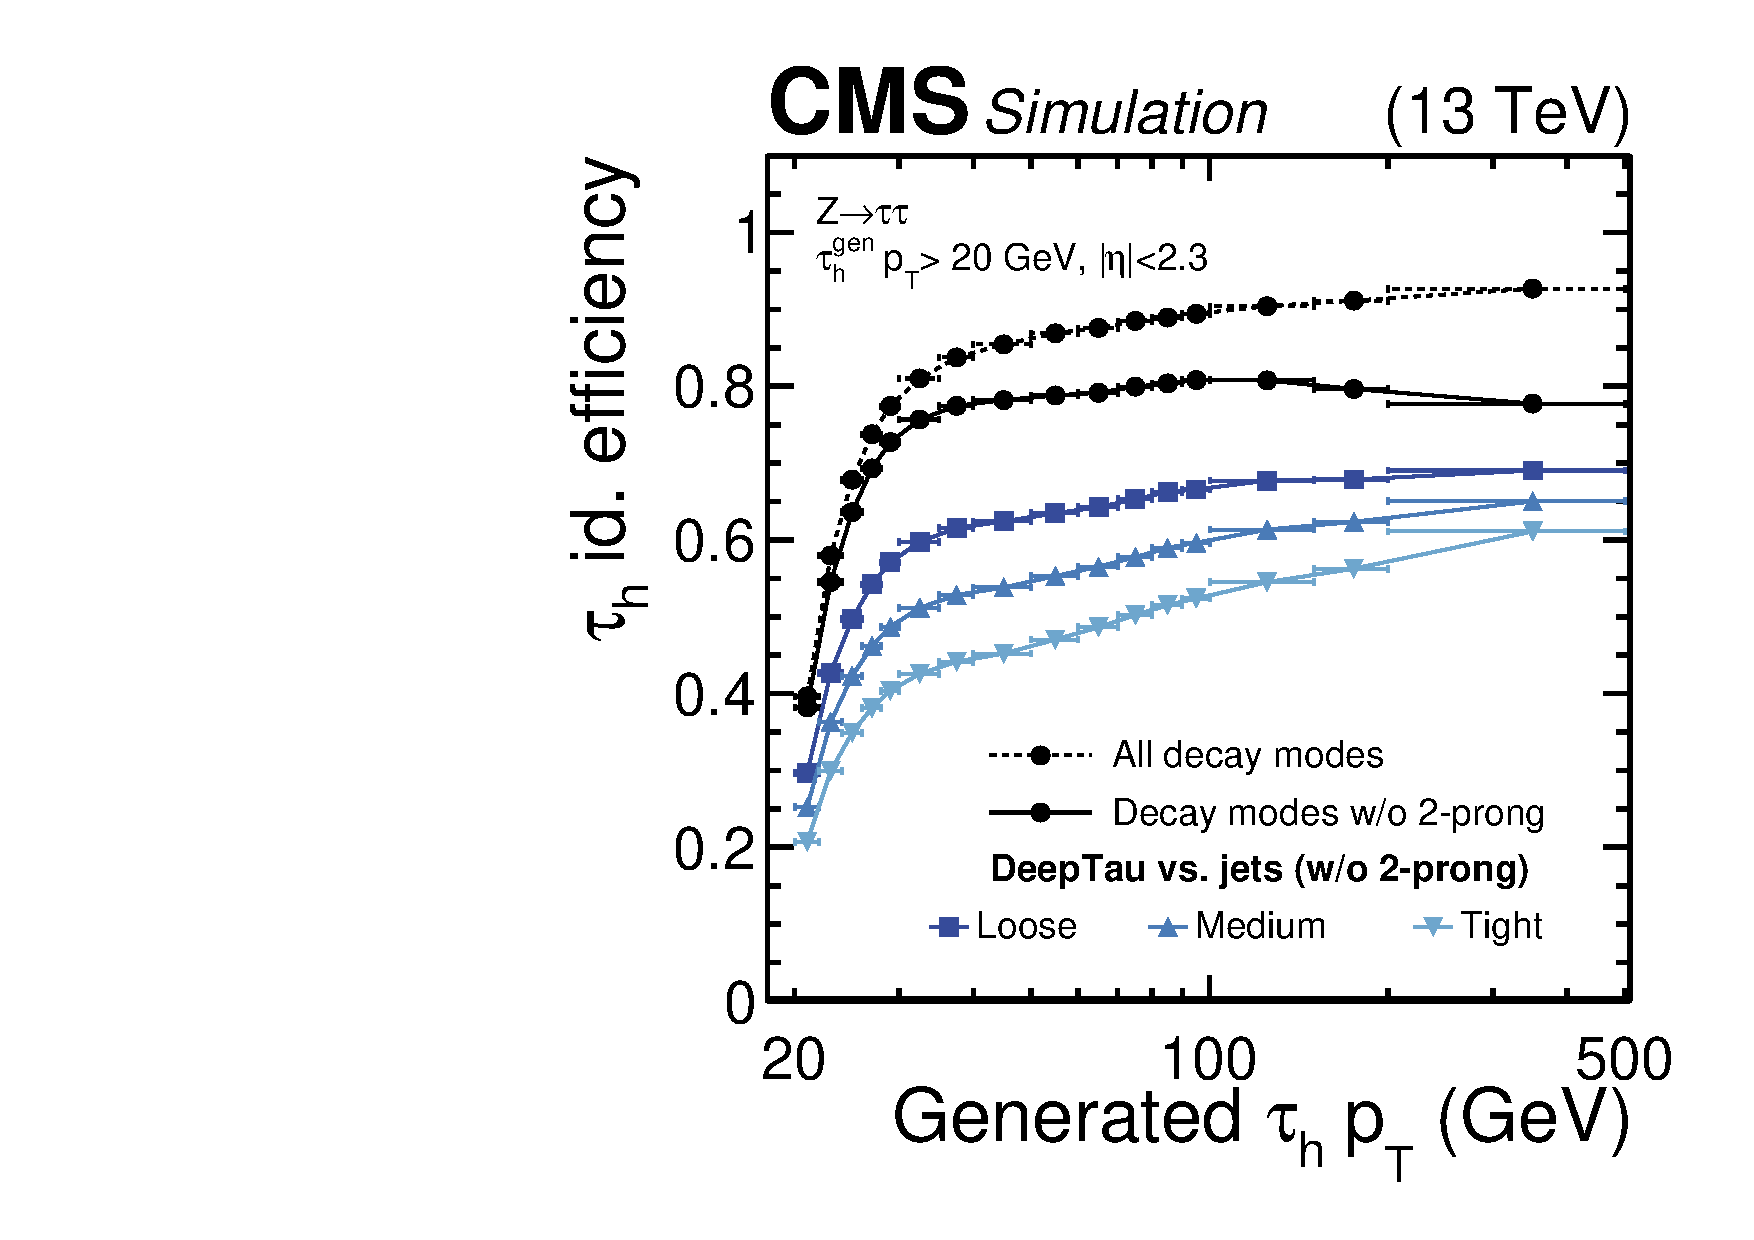
\includegraphics[width=0.49\textwidth]{Figures/Detector/CMS/tau_reco_id_eff.pdf}
  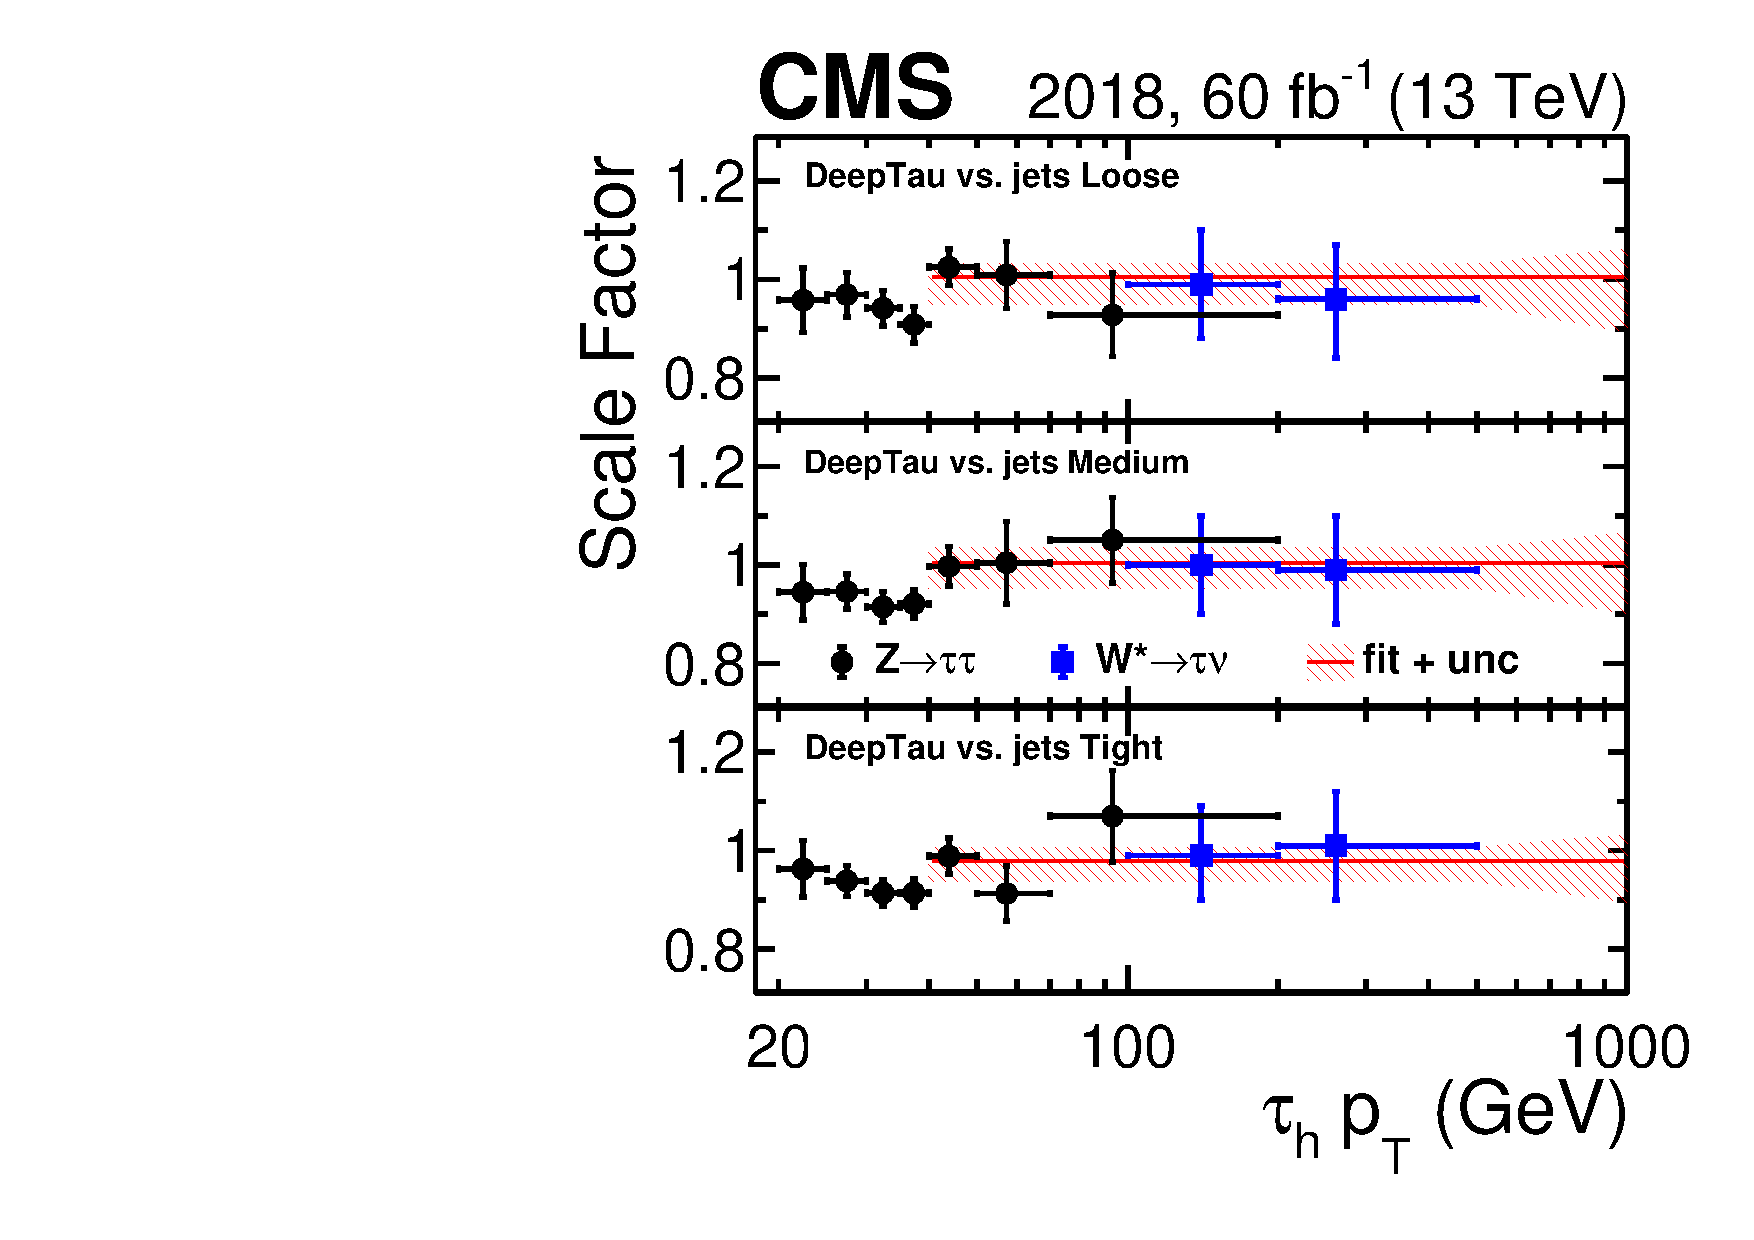
\includegraphics[width=0.49\textwidth]{Figures/Detector/CMS/tau_id_scale_factor.pdf}
  \caption[\tauh Reconstruction and Identification Efficiency]{Reconstruction and identification efficiency of \tauh candidates as measured in simulated $Z\to\tau\tau$ events (left) and corresponding scale factors measured with data collected in 2018 (right). In both plots, the results are shown as functions of the true (generated) \tauh \pt, and the efficiencies after applying the Loose, Medium and Tight DeepTau ID working points are calculated after excluding 2-prong decays, which are those containing missing charged hadrons. In the right plot, the vertical bars represent combined statistical and systematic uncertainties in the scale factors, and the red line and hatched region represents a constant fit to the scale factors for $\pt > 40$\GeV and the associated uncertainty. Figures taken from Ref.~\cite{CMS:2022prd}.}\label{fig:tau_reco_id_eff}
\end{figure}

\begin{figure}
  \centering
  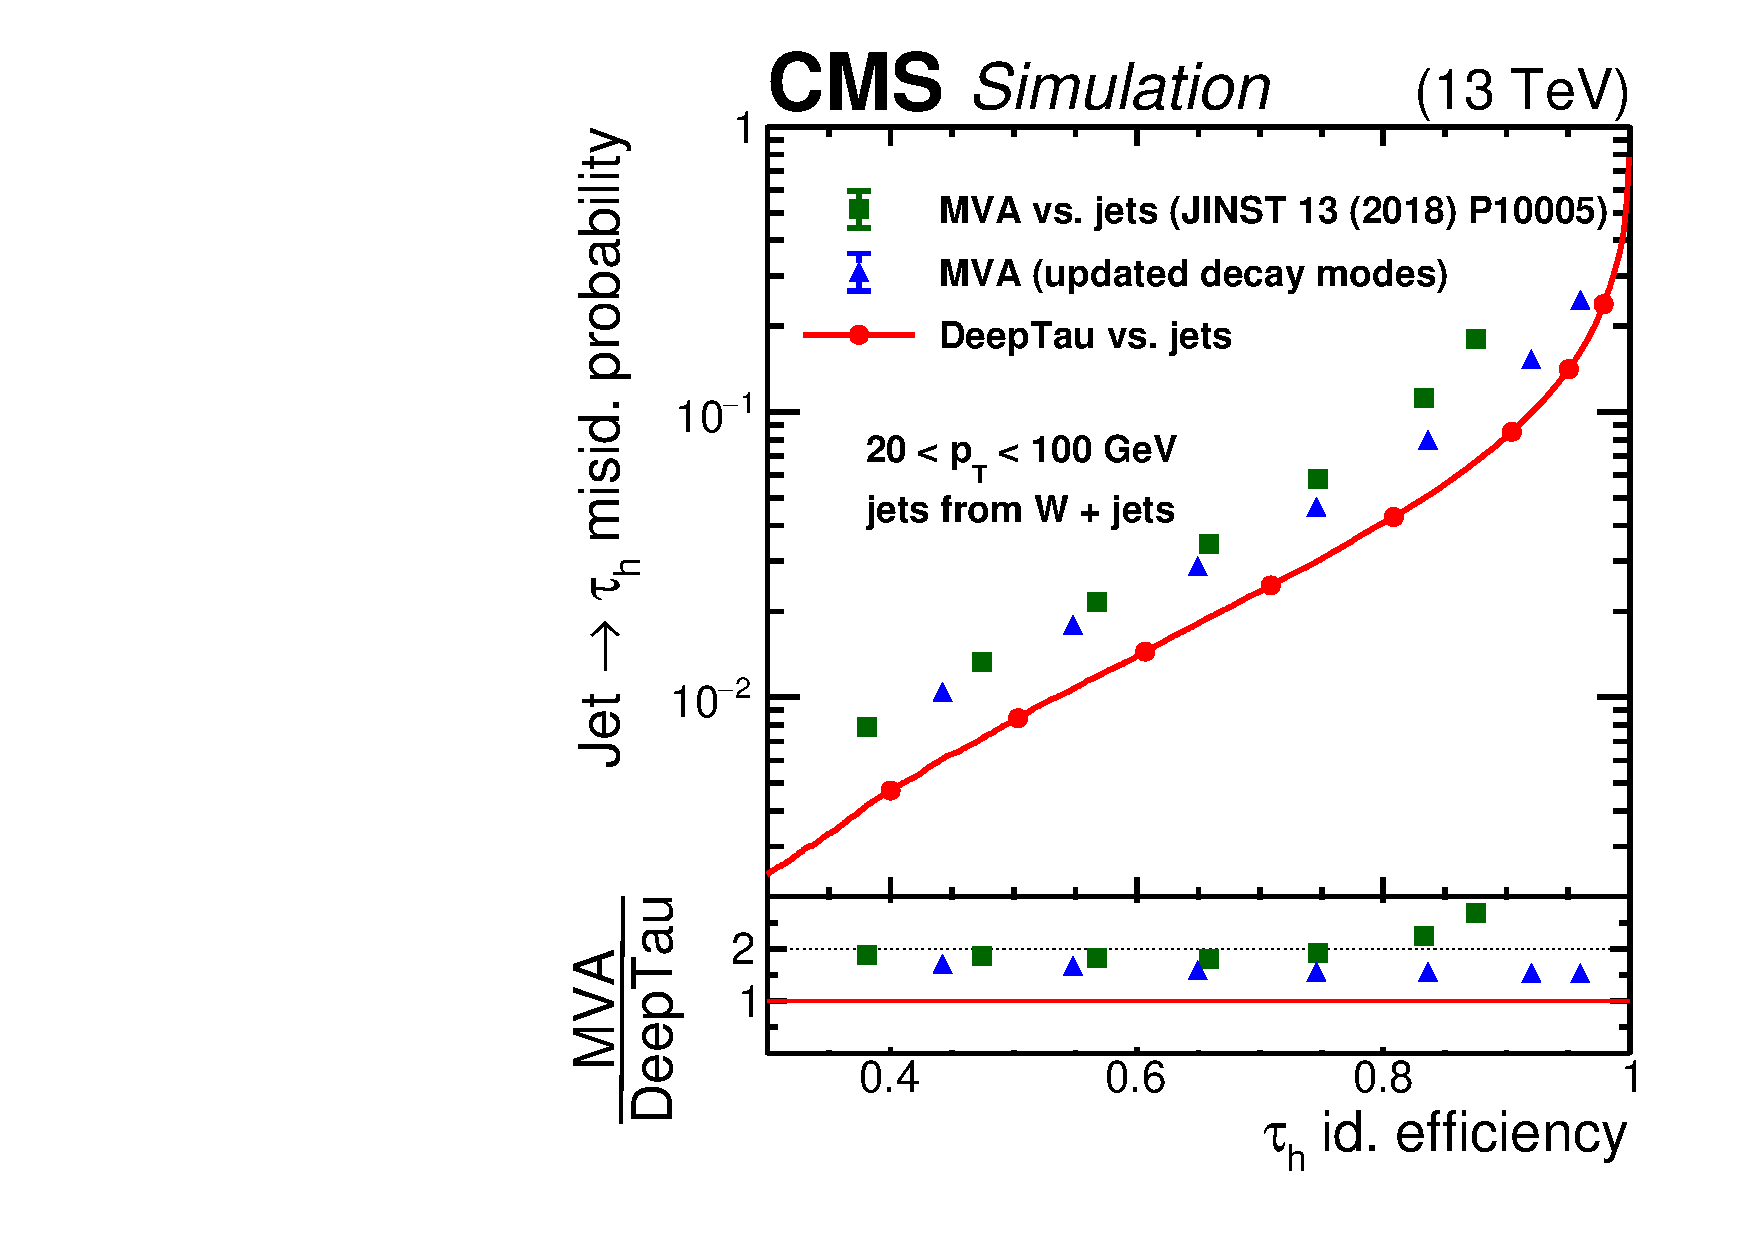
\includegraphics[width=0.49\textwidth]{Figures/Detector/CMS/tau_id_jet_misid_wjet_20_100.pdf}
  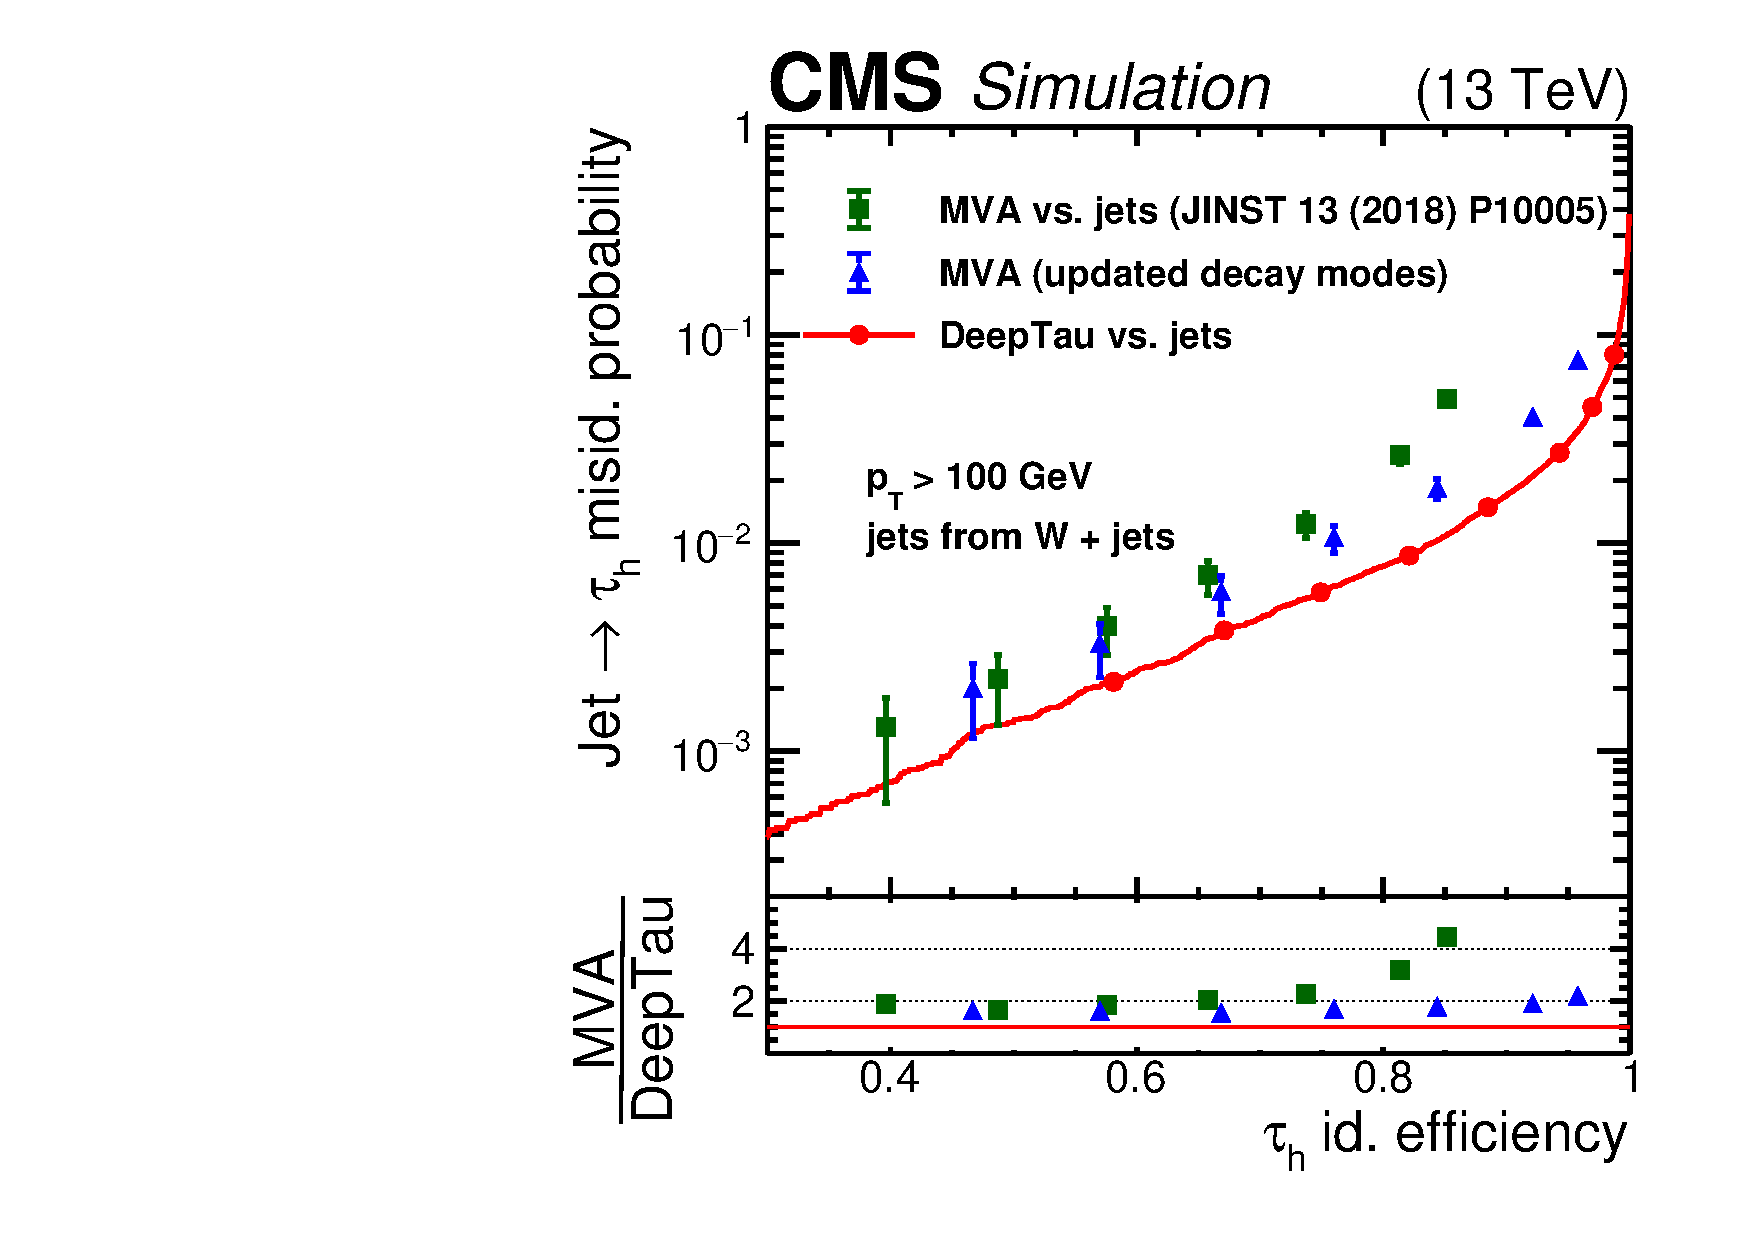
\includegraphics[width=0.49\textwidth]{Figures/Detector/CMS/tau_id_jet_misid_wjet_gt100.pdf}
  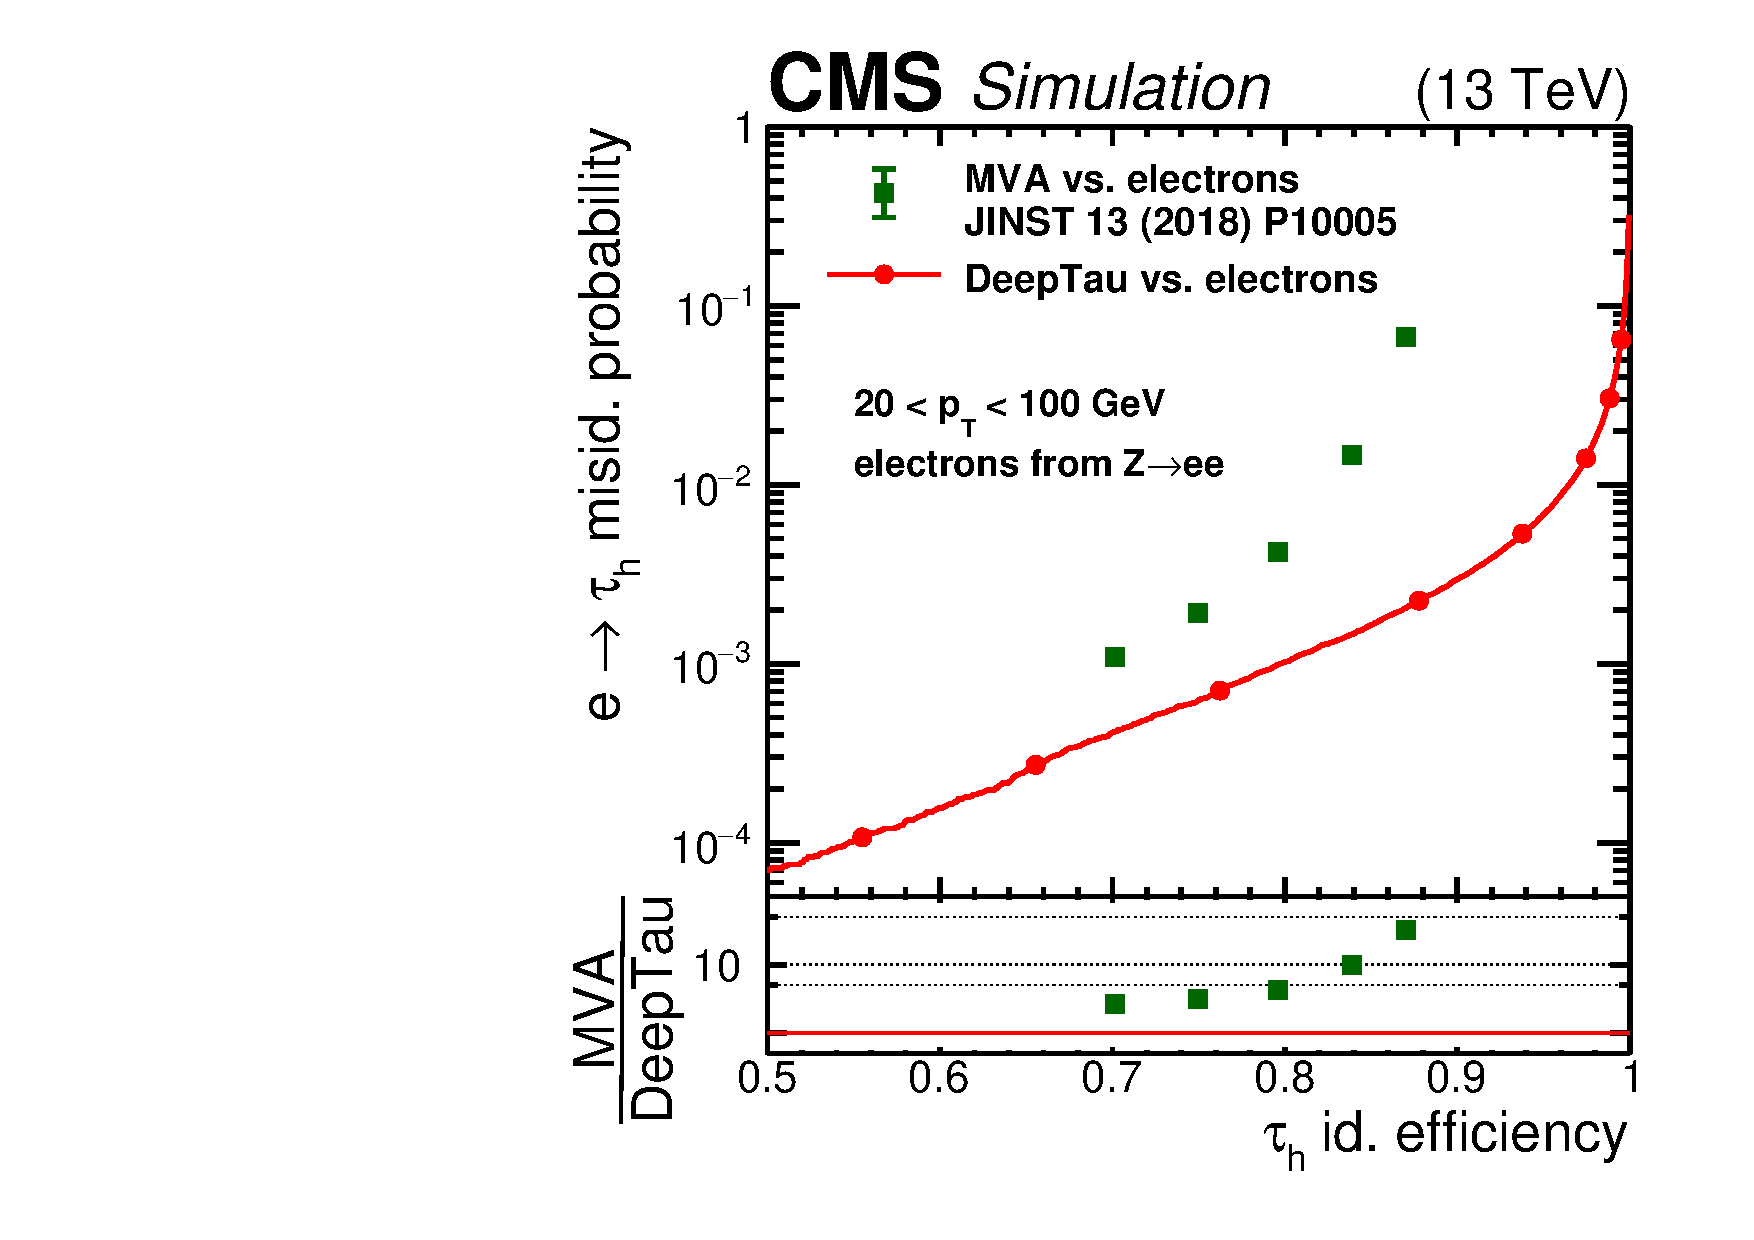
\includegraphics[width=0.49\textwidth]{Figures/Detector/CMS/tau_id_e_misid_20_100.pdf}
  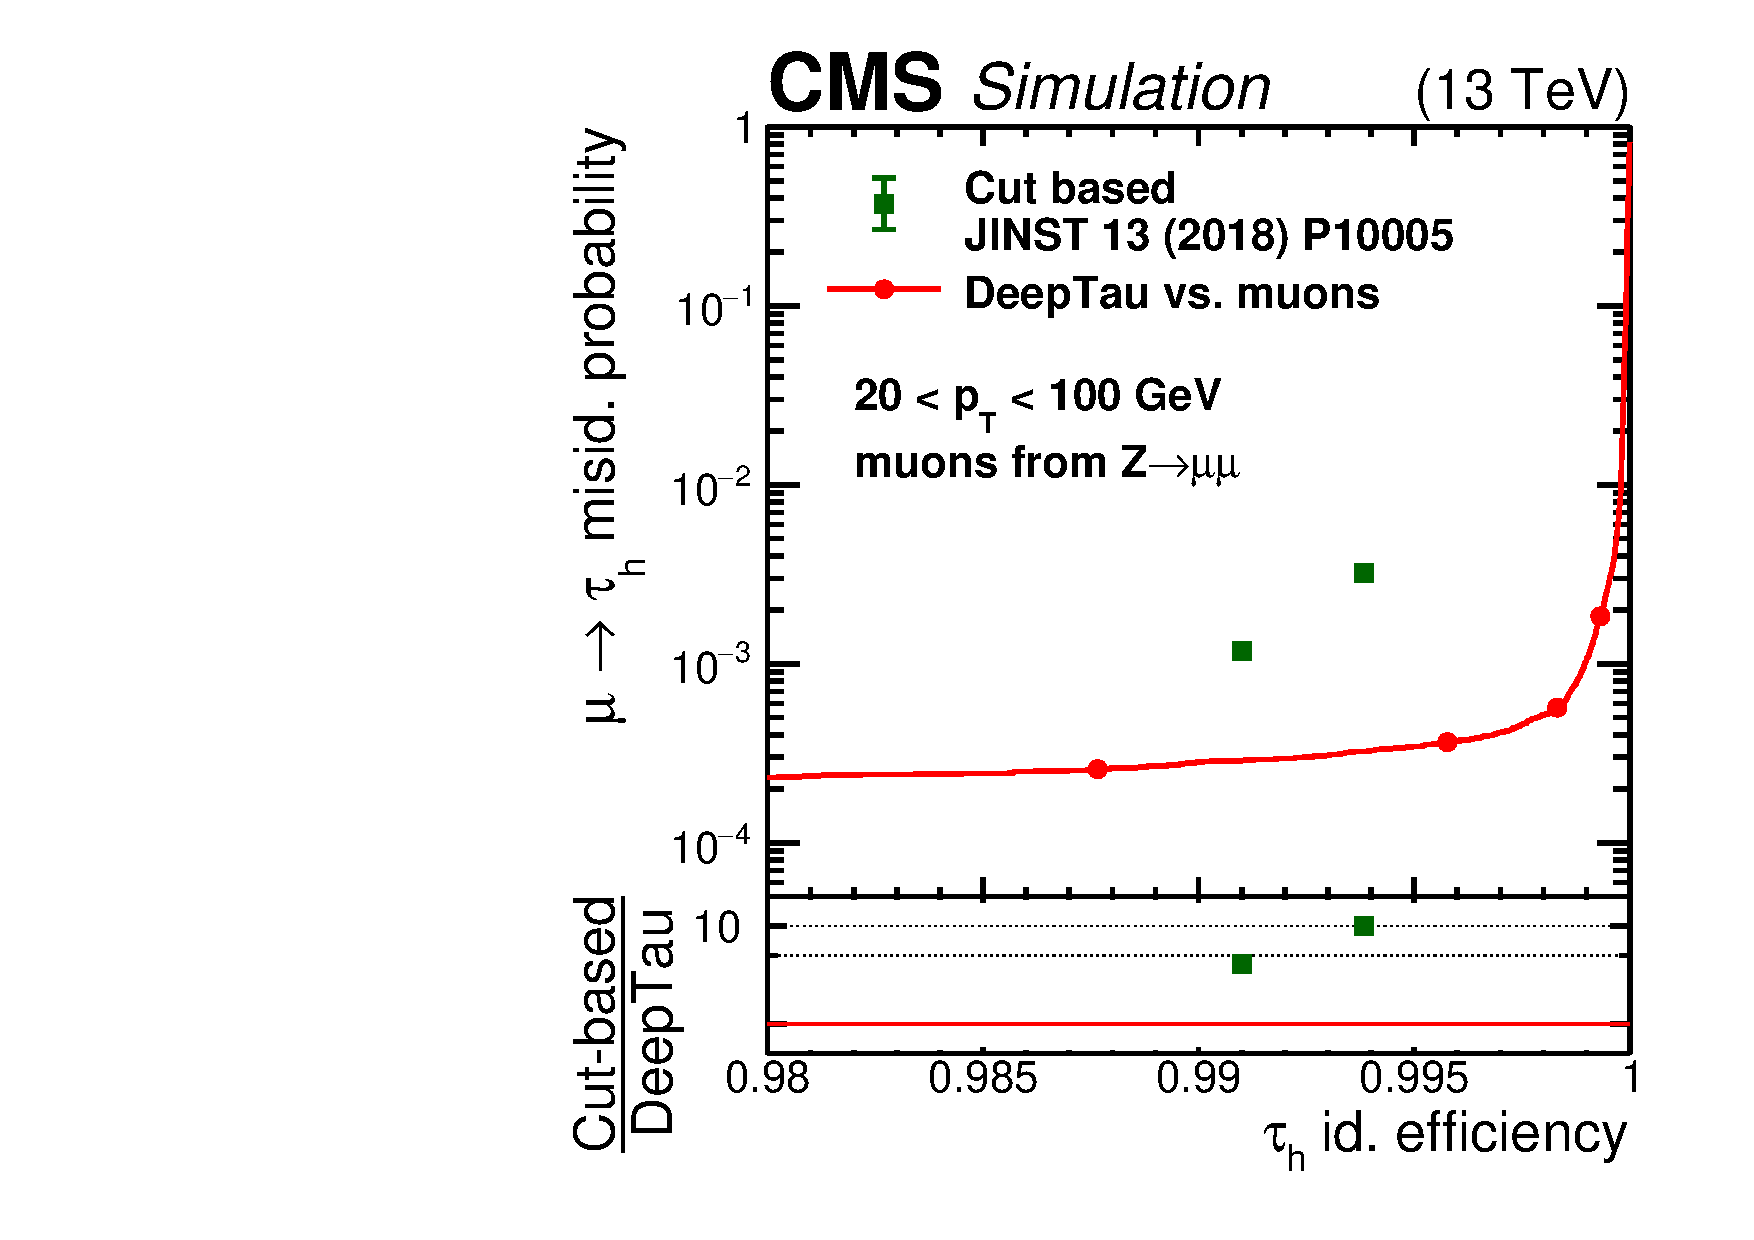
\includegraphics[width=0.49\textwidth]{Figures/Detector/CMS/tau_id_mu_misid_20_100.pdf}
  \caption[Performance of the DeepTau ID Algorithm]{Misidentification rates for jets (top), electrons (bottom left), and muons (bottom right) as a function of the \tauh identification efficiency for the \Djet, \De, and \Dm discriminators respectively. Also shown is the performance of previous \tauh identification algorithms and the ratio of misidentification rates between one of the alternate algorithms and DeepTau is shown in the bottom half of each plot. In all cases, DeepTau outperforms the alternate algorithm. For jets, efficiencies are shown for jets with $20 < \pt < 100$\GeV (top left) and $\pt>100$\GeV (top right) and they indicate that higher \pt jets are less likely to be misidentified. For electrons and muons, the efficiencies are only shown for $20 < \pt < 100$\GeV since the misidentification rate is approximately constant with \pt for these objects. Vertical bars represent statistical uncertainties and the full red circles represent the working points. Figures taken from Ref.~\cite{CMS:2022prd}.}\label{tab:deeptau_misid_rates}
\end{figure}

The \tauh reconstruction and identification efficiencies are also measured in data with $Z\to\mu\tauh$ and $W^*\to\nu\tauh$ events~\cite{CMS:2022prd} and scale factors are derived to correct the simulation to match data. These scale factors are derived in bins of \pt and their values and uncertainties are shown in \cref{fig:tau_reco_id_eff}. The corrections are at most 10\% and have an uncertainty of 2--5\%~\cite{CMS:2022prd}.

\subsubsection{\tauh Energy Scale}\label{sec:tau_energy_scale}

The \tauh energy scale is measured in data with $\mu\tauh$ events by fitting the distributions of the $\mu\tauh$ invariant mass, \mvis, and the reconstructed \tauh mass, \mtauh. Simulated templates of the \mvis and \mtauh distributions are created for \tauh energy shifts between $\pm3\%$ in steps of 0.2\% and a maximum likelihood fit is performed for each shift. This is performed in bins of the \tauh decay mode and separately for \mvis and \mtauh. The corresponding energy scale corrections are shown in \cref{fig:tau_energy_scale} and are found to be up to 2\% with uncertainties of 0.6--0.8\% depending on decay mode. The results from measuring \mvis and \mtauh are found to be consistent with each other and the final energy scale corrections are derived from a combination of the two approaches. After applying the corrections, good agreement is found in the \mvis and \mtauh distributions as shown in \cref{fig:tau_energy_scale_fit}.

\begin{figure}
  \centering
  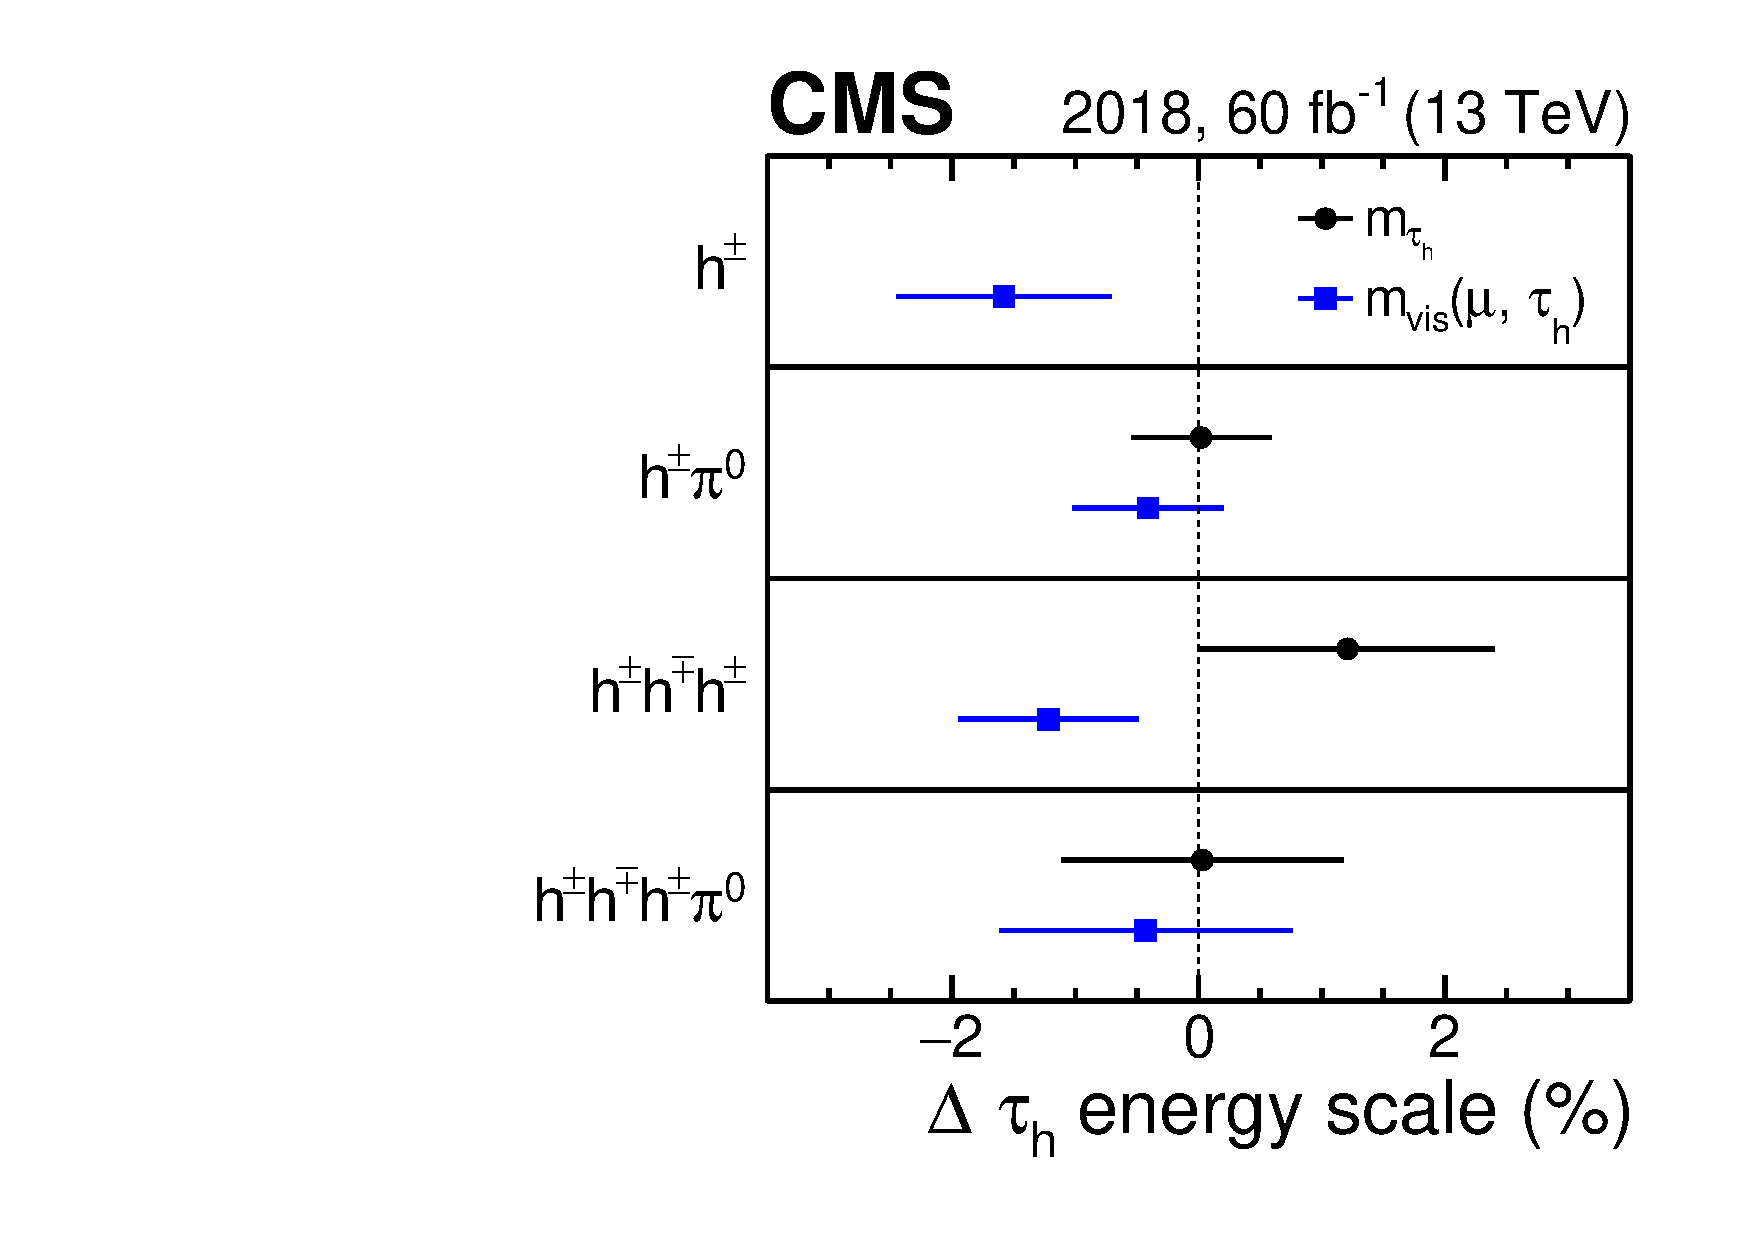
\includegraphics[width=0.5\textwidth]{Figures/Detector/CMS/tau_energy_scale.pdf}
  \caption[\tauh Energy Scale Corrections]{Relative difference for the \tauh energy obtained between data and simulated events for 2018 for the four main reconstructed \tauh decay modes. The results are obtained from fits to the distribution of either the reconstructed \mvis (blue lines) or \mtauh (black lines). The horizontal bars represent the combined statistical and systematic uncertainties in the measurements. Figure taken from Ref.~\cite{CMS:2022prd}.}\label{fig:tau_energy_scale}
\end{figure}

\begin{figure}
  \centering
  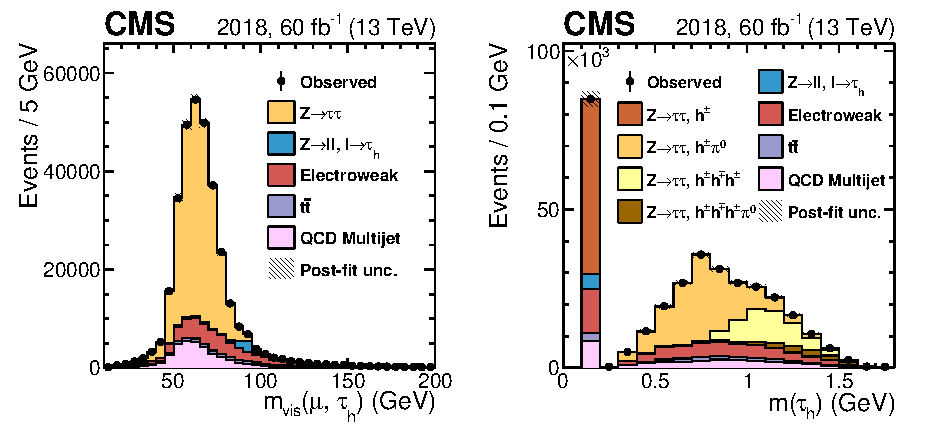
\includegraphics[width=\textwidth]{Figures/Detector/CMS/tau_energy_scale_fits.pdf}
  \caption[\tauh Energy Scale Agreement Between Simulation and Data]{Distribution of the reconstructed visible invariant mass of the $\mu\tauh$ system, \mvis (left) and of the visible invariant \tauh mass (right) in 2018 data (black dots) and simulated events (filled histograms). Vertical bars correspond to statistical uncertainties. The \tauh is required to pass the Tight \Djet working point, and have $\pt > 20$\GeV and $\abs{\eta}<2.3$. The distributions incorporate all measured scale factors and energy corrections and are scaled to the outcome of a maximum likelihood to the observed data with the $\PZ\to\tau\tau$ contribution freely floating. In the $m(\tauh)$ distribution, the $\PZ\to\tau\tau$ contributions are shown separately for the different \tauh decay modes. Figures taken from Ref.~\cite{CMS:2022prd}.}\label{fig:tau_energy_scale_fit}
\end{figure}

